\documentclass[9pt]{beamer}

\beamertemplatenavigationsymbolsempty
\renewcommand\mathfamilydefault{cmr}

\usepackage{xcolor}
\usepackage{pajmath}
\usepackage{booktabs}
\usepackage{colortbl}
\usepackage{tikz}
\usetikzlibrary{calc}
\usetikzlibrary{intersections}
\usetikzlibrary{datavisualization}
\usetikzlibrary{datavisualization.formats.functions}
\usepackage{pgfplots}

\newcommand\VW{\V{W}}
\newcommand\bsigma{\boldsymbol{\sigma}}
\newcommand\ytrue{y^\mathrm{true}}

\title{Neural Networks: Training and SGD}
\date{Spring 2021}

\begin{document}

\maketitle

\begin{frame}{Completing our matrix formalism}
\begin{center}
	\small
	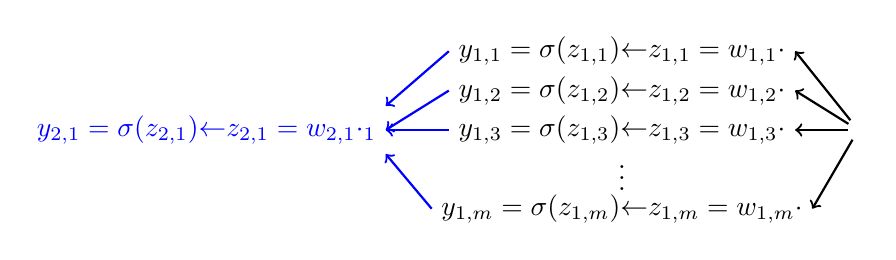
\begin{tikzpicture}
		\node (a) at (0,1.5) {$y_{1,1} =\sigma(z_{1,1}) \boldsymbol{\leftarrow} z_{1,1} = \V{w}_{1,1}\cdot\Vx$};
		\node (b) at (0,1) {$y_{1,2} =\sigma(z_{1,2}) \boldsymbol{\leftarrow} z_{1,2} = \V{w}_{1,2}\cdot\Vx$};
		\node (c) at (0,0.5) {$y_{1,3} =\sigma(z_{1,3}) \boldsymbol{\leftarrow} z_{1,3} = \V{w}_{1,3}\cdot\Vx$};
		\node (d) at (0,0) {$\vdots$};
		\node (e) at (0,-0.5) {$y_{1,m} =\sigma(z_{1,m}) \boldsymbol{\leftarrow} z_{1,m} = \V{w}_{1,m}\cdot\Vx$};
		\node (s) at (3,0.5) {$\Vx$};
		\draw [->,thick] (s) -- (a.east);
		\draw [->,thick] (s) -- (b.east);
		\draw [->,thick] (s) -- (c.east);
		\draw [->,thick] (s) -- (e.east);
		\node [blue,left] (o) at (-3,0.5) {$y_{2,1} =\sigma(z_{2,1}) \boldsymbol{\leftarrow} z_{2,1} = \V{w}_{2,1}\cdot\Vy_1$};
		\draw [->,blue,thick] (a.west) -- (o.north east);
		\draw [->,blue,thick] (b.west) -- (o.east);
		\draw [->,blue,thick] (c.west) -- (o.east);
		\draw [->,blue,thick] (e.west) -- (o.south east);
	\end{tikzpicture}
\end{center}

\pause
\[  \Vy_2 = \bsigma(\Vz_2) \quad\leftarrow\quad
	\Vz_2 = \V{W}_2\Vy_1 \quad\leftarrow\quad
	\Vy_1 = \bsigma(\Vz_1) \quad\leftarrow\quad
	\Vz_1 = \V{W}_1\Vx	 \]

\pause
\[ \Vy_2 = \bsigma(\V{W}_2(\bsigma(\V{W}_1\Vx))) \]

\pause
\bigskip
In general, a network with $d$ layers is
\[ \Vy_d = \bsigma(\V{W}_d(\bsigma(\V{W}_{d-1}(\cdots\bsigma(\V{W}_2(\bsigma(\V{W}_1\Vx))))))). \]

\end{frame}

\begin{frame}{Training neural networks}
We need two things to train neural networks:
\begin{enumerate}
	\item  loss function $L$ that measures how well the output of the final layer ($y_d$) compared with known training data.
	\item A set of training data $(\Vx_i,\ytrue_i)$.
\end{enumerate}

\bigskip
\pause
Let's assume we have some loss function $L$ that measures how well the output of the final layer ($y_d$) compared with known training data. For example, we could use quadratic loss
\[ L_i = (y_{d,i} - \ytrue_i)^2 \]

\bigskip
\pause
The loss function depends on all the weights in the network, i.e.\ $L_i(\V{W}_d,\V{W}_{d-1},\ldots,\V{W}_2,\V{W}_1)$. We will abbreviate this as simply $L_i(\V{W})$.

\end{frame}

\begin{frame}{Gradient descent}

We can use a gradient descent scheme to find the weights. Given an initial (random) set of weights $\VW^{(0)}$:
\begin{enumerate}
	\item Calculate the gradient of the \emph{total loss}
		\[ \V{g}(\VW) = \sum_{i=1}^N \dd{L_i(\VW)}{\VW}. \]
	\item Update the weights using
		\[ \VW^{(1)} = \VW^{(0)} - \alpha \V{g}(\VW^{(0)}). \]
	\item Repeat.
\end{enumerate}

\bigskip
\pause
The problem is the gradient calculation. 
\begin{itemize}
	\item The gradient has one entry for each parameter, of which there are thousands!
	\item These computations are repeated over all $N$ points in the dataset \emph{for each iteration}!
\end{itemize}

\end{frame}

\begin{frame}{Stochastic Gradient Descent (SGD)}

\addtolength{\itemsep}{0.5\baselineskip}
\begin{itemize}
	\item For neural network training we use an alternative to gradient descent called \emph{Stochastic Gradient Descent}, or SGD.
	\item SGD alternates between forward and backward passes through the model.
	\item SGD updates parameters using the loss for a single point.
	\item A single point provides a noisy, or \emph{stochastic} approximation to the true loss gradient, but it is far more efficient.
\end{itemize}

\end{frame}

\begin{frame}{The SGD algorithm}

\begin{enumerate}
	\item Select a single training point $(\Vx_i,\ytrue_i)$.
	\item Make a \textbf{forward pass} through the model to compute the output of the neural network
		\[ y_{d,i} = \bsigma(\V{W}_d(\bsigma(\V{W}_{d-1}(\cdots\bsigma(\V{W}_2(\bsigma(\V{W}_1\Vx_i))))))). \]
	\item Compute the loss for this single prediction
		\[ L_i = (y_{d,i} - \ytrue_i)^2. \]
	\item Calculate the gradient at this point and the current weights.
	\item Update the weights using
		\[ \VW^{(k+1)} = \VW^{(k)} - \alpha \V{g}(\VW^{(k)}). \]
		This completes the \textbf{backward pass}.
	\item Repeat for the next training point.
\end{enumerate}
	
\end{frame}

\begin{frame}{The SGD algorithm (simplified)}

\begin{enumerate}
	\item Select a single training point $(\Vx_i,\ytrue_i)$.
	\item Make a \textbf{forward pass} through the model to compute the output of the neural network
		\[ y_{d,i} \leftarrow \text{neural network} \leftarrow \Vx_i \]
	\item Compute the loss for this single prediction
		\[ L_i \leftarrow (y_{d,i},\, \ytrue_i) \]
	\item Calculate the gradient at this point and the current weights.
	\item Update the weights using
		\[ \dd{L_i}{\VW} \rightarrow \VW \]
		This completes the \textbf{backward pass}.
	\item Repeat for the next training point.
\end{enumerate}
	
\end{frame}

\begin{frame}{Implementing SGD}

\addtolength{\itemsep}{0.5\baselineskip}
\begin{itemize}
	\item Like gradient descent, SGD requires a step size hyperparameter ($\alpha$).
	\item One pass through the entire training set is called an \emph{epoch}.
	\item One epoch is not enough; often thousands are needed. The order of the training data is randomized between epochs.
	\item Some algorithms form \emph{minibatches} by averaging a small number of training samples before updating the weights.
\end{itemize}
	
\end{frame}

\begin{frame}{Why SGD?}

\addtolength{\itemsep}{0.5\baselineskip}
\begin{itemize}
	\item SGD is more efficient. Most datasets contain more points than are necessary to estimate the average, so computation is wasted.
	\item SGD is stochastic, just like the data. The stochasticity is a form of regularization.
	\item It just works, even if we don't understand why.
\end{itemize}
	
\end{frame}

\begin{frame}{How do neural networks learn so well?}

Neural network training \emph{should} get stuck in local optima, but it doesn't. There are three theories why:
\addtolength{\itemsep}{0.5\baselineskip}
\begin{enumerate}
	\item Lottery ticket theory: A good network is already somewhere in the randomly-initialized network.
	\item There are no true local optima in high-dimensional spaces.
	\item The noise in SGD allows training to ``escape'' local optima.
\end{enumerate}

\end{frame}

\begin{frame}{What else can we do to improve training?}

\addtolength{\itemsep}{0.5\baselineskip}
\begin{enumerate}
	\item \textbf{Regularize}. Neural networks can memorize anything, so we need to regularize them aggressively.
	\item \textbf{Boosting}. Train in several rounds, weighting the loss function toward points that are not predicted correctly.
	\item \textbf{Bagging}. Split the training data into parts and train a separate model on each part. Average the predictions of all the models.
	\item \textbf{Experiment}. Change number and size of layers, hyperparameters, optimizers, batching, and regularization.
\end{enumerate}

\end{frame}


\end{document}
